
\documentclass[10pt,a4paper]{report}
\usepackage[utf8]{inputenc}
\usepackage[russian]{babel}
\usepackage{amsmath}
\usepackage{amsfonts}
\usepackage{amssymb}
\usepackage{graphicx}
\usepackage{listings}

\usepackage[left=1.8cm, right=1cm, top=0.8cm, bottom=2cm, 
bindingoffset=0cm]{geometry}

\author{Климов Сергей}
\title{Лабораторная работа №6.\\
	SSL/TLS}
\begin{document}
	\maketitle
	\renewcommand{\thesection}{\arabic{section}}
	\tableofcontents
	\pagebreak
	
	\setcounter{totalnumber}{10}
	\setcounter{topnumber}{10}
	\setcounter{bottomnumber}{10}
	\renewcommand{\topfraction}{1}
	\renewcommand{\textfraction}{0}
	
	\section{Цель работы}
	\begin{itemize}
		\item Изучить лучшие практики по развертыванию SSL/TLS.
		\item Изучить основные уязвимости и атаки на SSL последнего времени - POODLE, HeartBleed.
	\end{itemize}
	
	\section{Изучение практик по развертыванию SSL/TLS}
		\begin{itemize}
			\item Использование 2048-битных закрытых ключей, например:
			\begin{itemize}
				\item 2048-битный RSA 
				\item 256-битные ECDSA закрытые ключи.
			\end{itemize}
			
		\item Необходимо защищать закрытые ключи, предоставляя доступ к ним как можно меньшему числу сотрудников. Рекомендуемые меры:
		\begin{itemize}
				\item Генерируйте закрытые ключи и запросы на сертификат (CSRs) на доверенном компьютере. Некоторые CA предлагают генерацию ключей и CSRs для вас, но это нецелесообразно.

				\item Используйте парольную защиту закрытых ключей, чтобы предотвратить их компрометацию в тех случаях, когда они хранятся в резервных системах. Парольная защита закрытых ключей не помогает на промышленном сервере, потому что злоумышленник может получить ключи из процесса памяти. Есть аппаратные устройства, которые могут защитить секретные ключи даже в случае компрометации сервера, но они стоят дорого и, таким образом, оправданы только в организациях с высокими требованиями безопасности.

				\item После компрометации отзывайте старые сертификаты и генерируйте новые ключи.

				\item Обновляйте сертификаты каждый год и всегда с новыми закрытыми ключами.
			\end{itemize}		
			
			\item Необходимо обеспечить охват всех используемых доменных имен, 
			которые будут использоваться.
			
			\item Приобретение сертификатов у надежного удостоверяющего центра.
			
			\item Использование надежных алгоритмов подписи сертификата.
			
			\item Использование безопасных протоколов, например TLS v1.0 - TLS v1.2.
			
			\item Использование безопасных алгоритмов шифрования, т.е. только те алгоритмы шифрования, которые обеспечивают аутентификацию и шифрование в 128 бит или более.
			
			\item Контроль выбора алгоритма шифрования.
			В SSL версии 3 и более поздних версиях протокола, клиенты отправляют 
			список алгоритмов шифрования, которые они поддерживают, и сервер выбирает 
			один из них для организации безопасного канала связи.
			Не все сервера могут делать это хорошо, так как некоторые выбирают первый 
			поддерживаемый алгоритм из списка.
			Таким образом, выбор правильного алгоритма шифрования является критически 
			важным для безопасности.
			
			\item Поддержка Forward Secrecy.
			Forward Secrecy — это особенность протокола, который обеспечивает 
			безопасный обмен данными, он не зависит от закрытого ключа сервера.
			С алгоритмами шифрования, которые не поддерживают Forward Secrecy, 
			возможно расшифровать ранее зашифрованные разговоры с помощью закрытого 
			ключа сервера.
			Нужно поддерживать и предпочитать ECDHE алгоритмы шифрования.
			Для поддержки более широкого круга клиентов, вы должны также использовать 
			DHE, как запасной вариант после ECDHE.
		\end{itemize}
	\section{Уязвимости POODLE и HeartBleed}
		\begin{itemize}
			\item POODLE (CVE-2014-3566) - Для получения доступа к данным злоумышленники вначале должны эмулировать несовместимость реализаций защищенного соединения между клиентом и сервером для того, чтобы клиентское ПО инициировало переход от более безопасных протоколов TLS на уровень SSL 3.0 – т.н. “downgrade dance”. После этого у злоумышленников появляется возможность получить доступ к критичной информации – например, к заголовкам, которые хранят в cookie авторизационную информацию. Атака возможна по схеме Man in the middle – хакер должен перехватывать информацию между клиентом и сервером и иметь возможность модифицировать ее.
			
			\item Heartbleed (CVE-2014-0160) - ошибка (переполнение буфера) в 
			криптографическом программном обеспечении OpenSSL, позволяющая 
			несанкционированно читать память на сервере или на клиенте, в том числе 
			для извлечения закрытого ключа сервера. 
			Heartbleed осуществляется отправкой некорректно сформированного 
			Heartbeat-запроса, в котором реальный размер строки очень мал, а число, 
			символизирующее длину передаваемой строки, очень велико.
			Так можно получить в ответ от сервера больше всего скрытой информации.
			Таким образом, у жертвы возможно за один запрос узнать до 64 килобайт 
			памяти, которая была ранее использована OpenSSL.
		\end{itemize}
	
	\section{Изучение отчетов ресурса SSL Server Test}
		\subsection{Домен из раздела Recent Best}
			В качестве домена из раздела Recent Best был выбран домен black-khat.com (203.7.2.247).
			Отчет представлен на рисунке~\ref{ris:site1}.

			\begin{figure}[h]
				\centering
				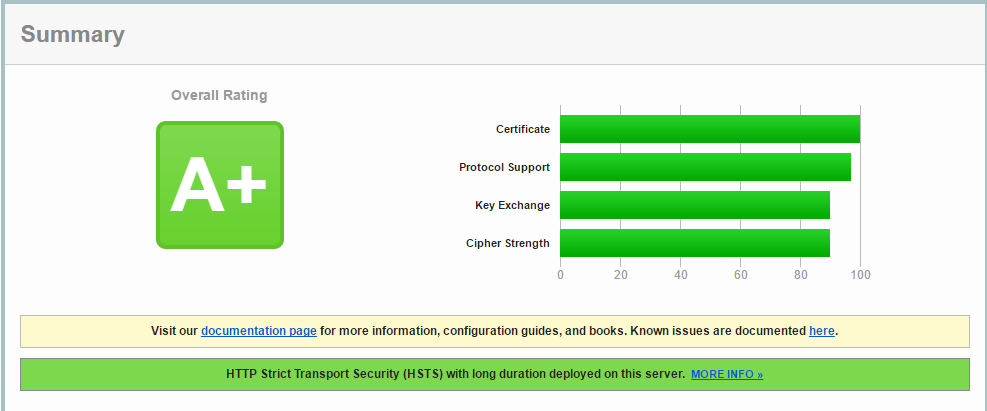
\includegraphics[width=0.9\textwidth]{imgs/1.png}
				\caption{Отчет для сайта black-khat.com}
				\label{ris:site1}
			\end{figure}

		Данный сервер поддерживает длительное форсированное защищенное соединение через HTTPS, что позволяет сразу же устанавливать безопасное соединение, вместо использования HTTP-протокола. Механизм использует особый заголовок Strict-Transport-Security для принудительного использования браузером протокола HTTPS даже в случае перехода по ссылкам с явным указанием протокола HTTP. 
			
			В качестве домена из раздела Recent Worst был выбран домен 
secure.ecommerce.aliant.net (142.166.145.159).
			Отчет представлен на рисунке~\ref{ris:site2}.

			\begin{figure}[h]
				\centering
				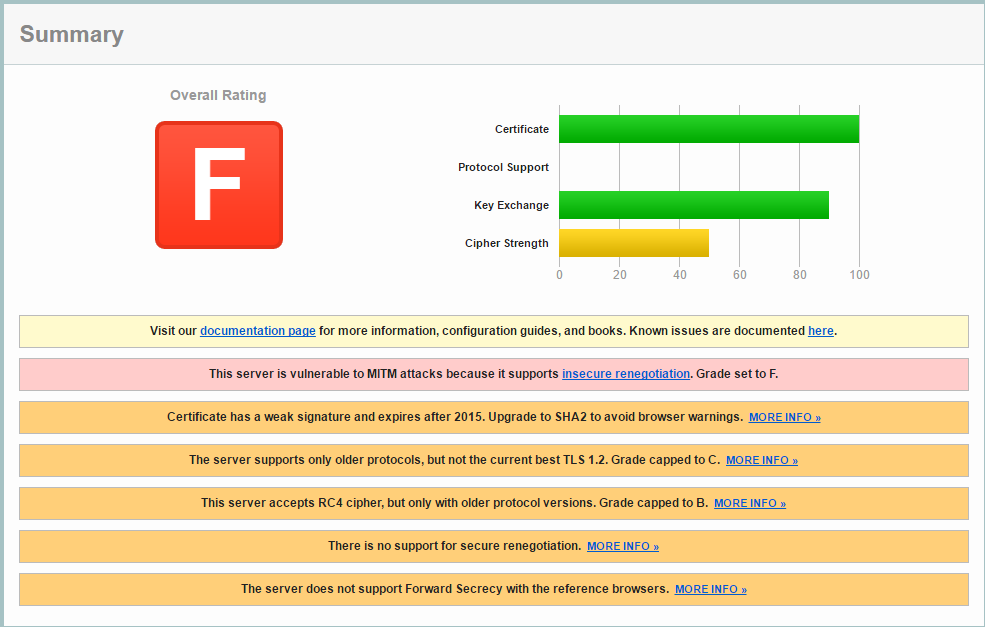
\includegraphics[width=0.9\textwidth]{imgs/2.png}
				\caption{Отчет для сайта secure.ecommerce.aliant.net}
				\label{ris:site2}
			\end{figure}
	
			\begin{itemize}
				\item Этот сервер подвержен MITM атакам;
				\item Сертификат имеет слабое шифрование подписи и истекает после 2015г.
				\item Сервер поддерживает только старые протоколы TLS, а не современную его версию - 1.2.
				\item Этот сервер принимает шифр RC4, но только с более старыми версиями протокола.
				\item Сервер не поддерживает Forward Security для браузеров.
			\end{itemize}
			
			Для самостоятельного анализа был выбран сервер bankofamerica.com (171.161.148.150).
			Результаты анализа приведены на рисунке~\ref{ris:site3}

			\begin{figure}[h]
				\centering
				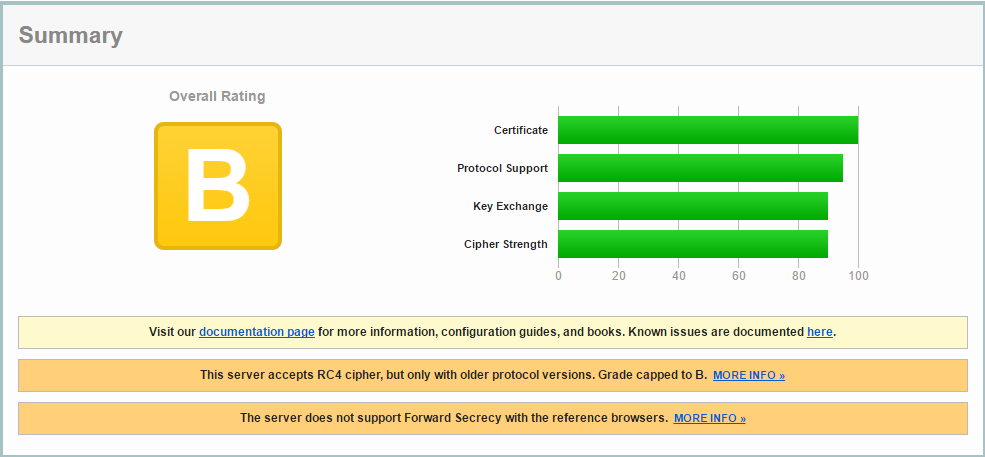
\includegraphics[width=0.9\textwidth]{imgs/3.png}
				\caption{Отчет для сайта bankofamerica.com }
				\label{ris:site3}
			\end{figure}
		
			Как видно из рисунка~\ref{ris:site3}, сервис bankofamerica.com  поддерживает все 
			типы протоколов TLS, однако он принимает шифр RC4 только с более старыми версиями протокола и не поддерживает Forward Security для браузеров.
			
		\subsection{Расшифровка аббревиатур}
			Аббревиатуры представлены ниже:
			\begin{lstlisting}
TLS_RSA_WITH_AES_256_CBC_SHA256 (0x3d)	256
TLS_RSA_WITH_AES_256_CBC_SHA (0x35)	256
TLS_RSA_WITH_AES_128_CBC_SHA256 (0x3c)	128
TLS_RSA_WITH_AES_128_CBC_SHA (0x2f)	128
TLS_RSA_WITH_3DES_EDE_CBC_SHA (0xa)	112
TLS_RSA_WITH_RC4_128_SHA (0x5)   INSECURE	128
TLS_ECDHE_RSA_WITH_AES_256_CBC_SHA384 (0xc028)   ECDH secp256r1 (eq. 3072 bits RSA)   FS	256
TLS_ECDHE_RSA_WITH_AES_256_CBC_SHA (0xc014)   ECDH secp256r1 (eq. 3072 bits RSA)   FS	256
TLS_ECDHE_RSA_WITH_AES_128_CBC_SHA256 (0xc027)   ECDH secp256r1 (eq. 3072 bits RSA)   FS	128
TLS_ECDHE_RSA_WITH_AES_128_CBC_SHA (0xc013)   ECDH secp256r1 (eq. 3072 bits RSA)   FS	128
TLS_ECDHE_RSA_WITH_3DES_EDE_CBC_SHA (0xc012)   ECDH secp256r1 (eq. 3072 bits RSA)   FS
			\end{lstlisting}
			
			Расшифровка аббревиатур:
			\begin{itemize}
				\item TLS\_ECDHE - алгоритм Диффи-Хэлмана на эллиптических кривых;
				\item RSA - алгоритм шифрования с открытым ключем;
				\item AES\_128 - алгоритм шифрования с длиной ключа в 128 бит;
				\item GCM и CBC - режимы блочного шифрования;
				\item SHA256 - хэш-функция с длиной ключа 256 бит.
			\end{itemize}
			
		\subsection{Описание позиций в разделе Protocol Details}
			Содержимое раздела Protocol Details представлено ниже:
			\begin{itemize}
				\item Проверка сертификата:
				\begin{lstlisting}
Secure Renegotiation	Supported
Secure Client-Initiated Renegotiation	No
Insecure Client-Initiated Renegotiation	No
				\end{lstlisting}
				
				\item Уязвимость к атакам Poodle, Bcast, Downgrade
				\begin{lstlisting}
BEAST attack	Not mitigated server-side (more info)   TLS 1.0: 0xc035
POODLE (SSLv3)	No, SSL 3 not supported (more info)
POODLE (TLS)	No (more info)
Downgrade attack prevention	Yes, TLS_FALLBACK_SCSV supported (more info)
				\end{lstlisting}
				
				\item Используется слабый алгоритм RC4
				\begin{lstlisting}
RC4	Yes   INSECURE (more info)
				\end{lstlisting}
				
				\item Сервер защищен от атак HeartBleed
				\begin{lstlisting}
Heartbeat (extension)	No
Heartbleed (vulnerability)	No (more info)
				\end{lstlisting}
				
				\item Совместимость Forward Security с браузерами
				\begin{lstlisting}
Forward Secrecy	With some browsers (more info)
				\end{lstlisting}
				
				\item Не поддерживает ALPN и NPN
				\begin{lstlisting}
ALPN	No
NPN	No
				\end{lstlisting}
				
				\item Параметры сессии.
				\begin{lstlisting}
Session resumption (caching)	No (IDs assigned but not accepted)
Session resumption (tickets)	No
				\end{lstlisting}
				
				\item Реализация HSTS.
				\begin{lstlisting}
Strict Transport Security (HSTS)	No
HSTS Preloading	Not in: Chrome  Edge  Firefox  IE  Tor 
				\end{lstlisting}
				
				\item Реализация HPKP (отсутствует).
				\begin{lstlisting}
Public Key Pinning (HPKP)	No
				\end{lstlisting}
				
				\item Совместимость с SSL2 (совместим).
				\begin{lstlisting}
SSL 2 handshake compatibility	Yes
				\end{lstlisting}
			\end{itemize}
		
		\subsection{Вывод о реализации SSL на выбранном домене}
			Исходя из отчета, сервис bankofamerica.com имеет среднюю защищенность:
			использует доверенный сертификат и защищен от основных типов атак, однако сервер использует устаревший алгоритм RC4, который является 
уязвимым. Так же сервис имеет поддержку Forward Security для большинства браузеров.
		
	\section{Выводы}

		В данной лабораторной работе было произведено озакомление с сервисом проверки защищенности серверов Qualys SSLLABS и рассмотрены последние самые опасные уязвимости: POODLE и HeartBeat.
		Были рассмотрены отчеты по безопасности различных серверов с разными рейтингами.
		Были рассмотрены основные параметры, которые сервис прверяет на предмет защищенности сервера, их существует достаточно большое количество, поэтому настоить сервер на использование безопасного соединения с должной степенью защищенности является нетривиальной задачей.
	
\end{document}